% !TEX root = PREN2_Dokumentation.tex
\section{Methoden}
\subsection{\gls{SoDa}}
Das Projektmanagement wird mit dem hybriden Projektvorgehen \gls{SoDa} der Hochschule Luzern durchgeführt. 
SoDa wurde dabei bereits schon in vorhergehenden Softwareentwicklungsmodulen eingesetzt und hat sich hier bewährt. Die Userstories werden dabei auch im \gls{GitLab} erfasst.  
\begin{figure}[H]
	\centering
	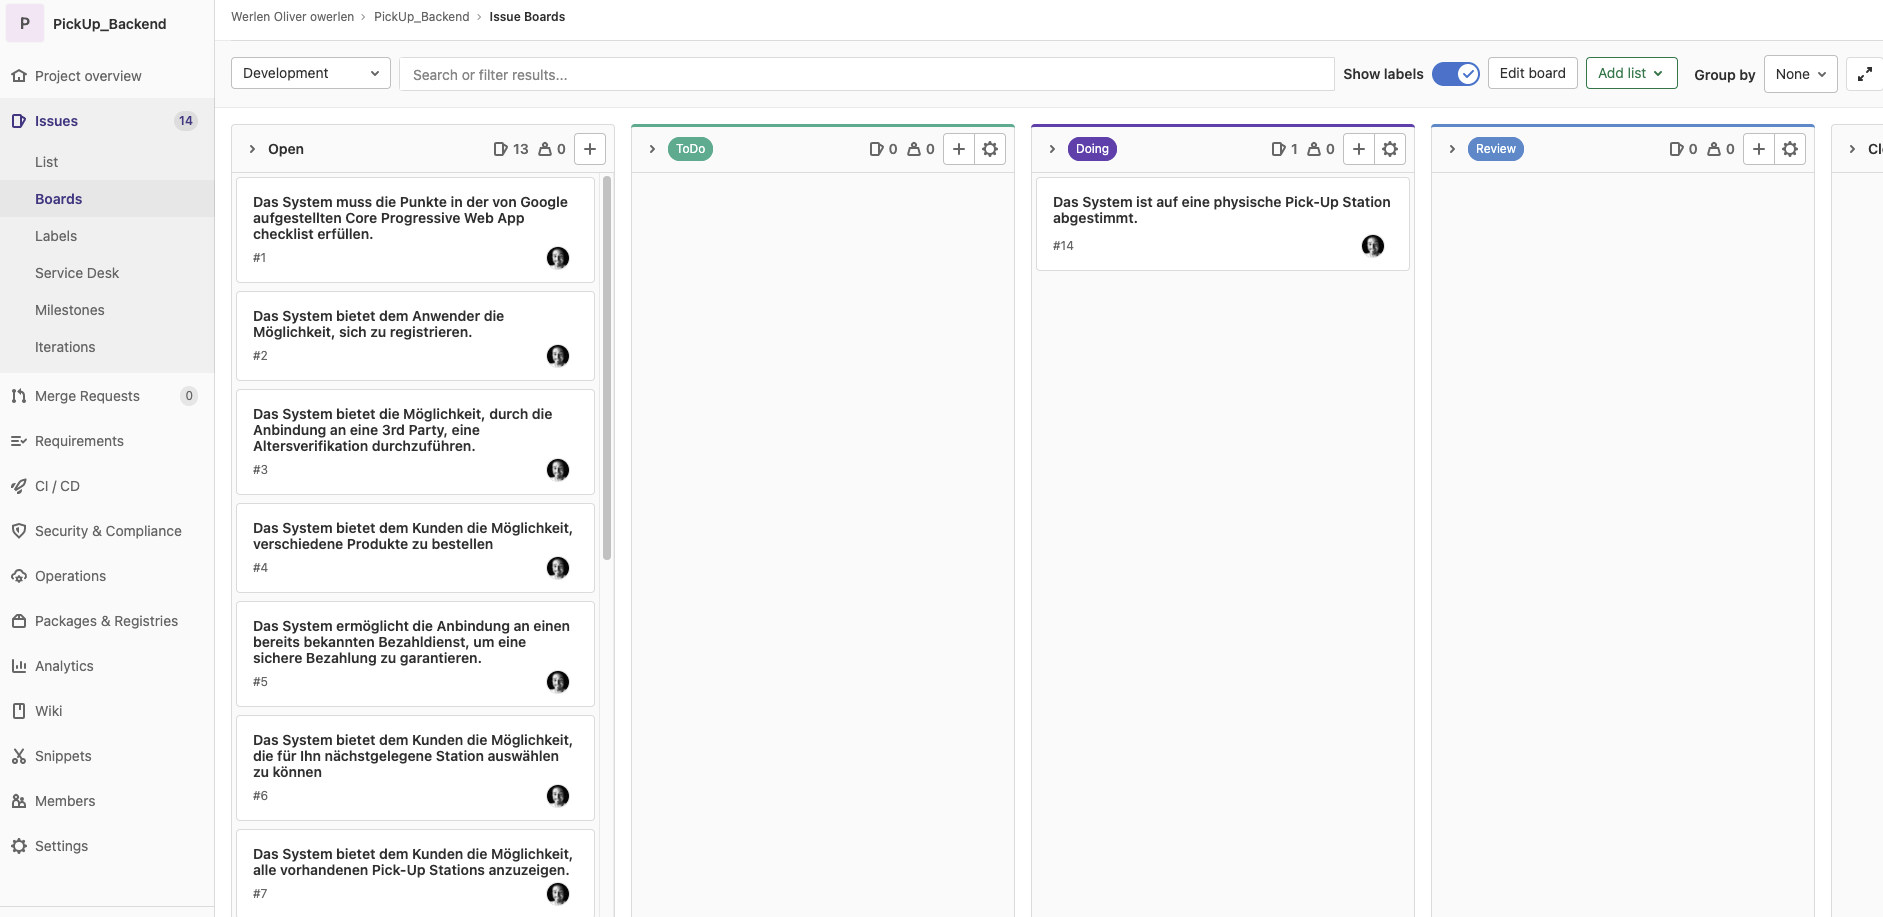
\includegraphics[width=1\textwidth]{images/boardGitlab.png}
	\caption[GitLab Board]{GitLab Board,\\ Quelle: Autor}
	\label{img: GitlLabBoard}
\end{figure}
Für die Sprint Planung werden einzelne User Stories verschoben. Beim Sprint Review werden die Stories in "reviewing" mit den definierten Akzeptanzkriterien mit den Resultaten verglichen. Basierend darauf wird entschieden, ob an der \gls{User Story} noch weiter gearbeitet werden, das heisst zurück zu "doing" oder die Story in "done" verschoben werden kann. Bei Beginn des nächsten Sprints wird das Vorgehen wiederholt. \\
Die einzelnen Items sind dabei priorisiert. Elemente mit einer hohen Einstufung werden dabei bei der Bearbeitung vorgezogen. 

\subsection{CI/CD}
Die gesamte \ac{CI/CD} Pipeline wurde für dieses Projekt neu erstellt. Dabei besteht der Prozess aus drei Stages: 
\begin{enumerate}
	\item build
	\item package
	\item deploy
\end{enumerate}

\subsubsection{build}
Abhängig vom Projekt wird das Projekt gebuilded. Bei der Java Applikation handelt es sich hier um ein maven-package, beim Angular Frontend um ein ng build --prod. Die resultierenden Artifakte werden für zwei Stunden im GitLab gespeichert. 
\subsubsection{package}
In der Package Stage wird das Docker Image aus den vorherigen Artifakten erstellt. Dabei wird das Dockerfile des jeweiligen Produkts genutzt. Der Build wird von einem Shared Runner durchgeführt. Hier werden 4 vom Enterpriselab zur Verfügung gestellt. Anschliessend wird dieses in die Container Registry des GitLab Projekts gepushed. 
\subsubsection{deploy}
Für das Deployment wurde auf den virtuellen Maschinen ein GitLab Runner installiert. Durch den deployment-Tag wird dieser adressiert. Auf diese Maschine wird ein Login ausgeführt und anschliessend das aktuellste Image heruntergeladen. Es wird der bestehende Container gelöscht und aus dem neuen Image ein neuer Container gestartet. 

\subsubsection{Sequenzdiagramm}
\begin{figure}[H]
	\centering
	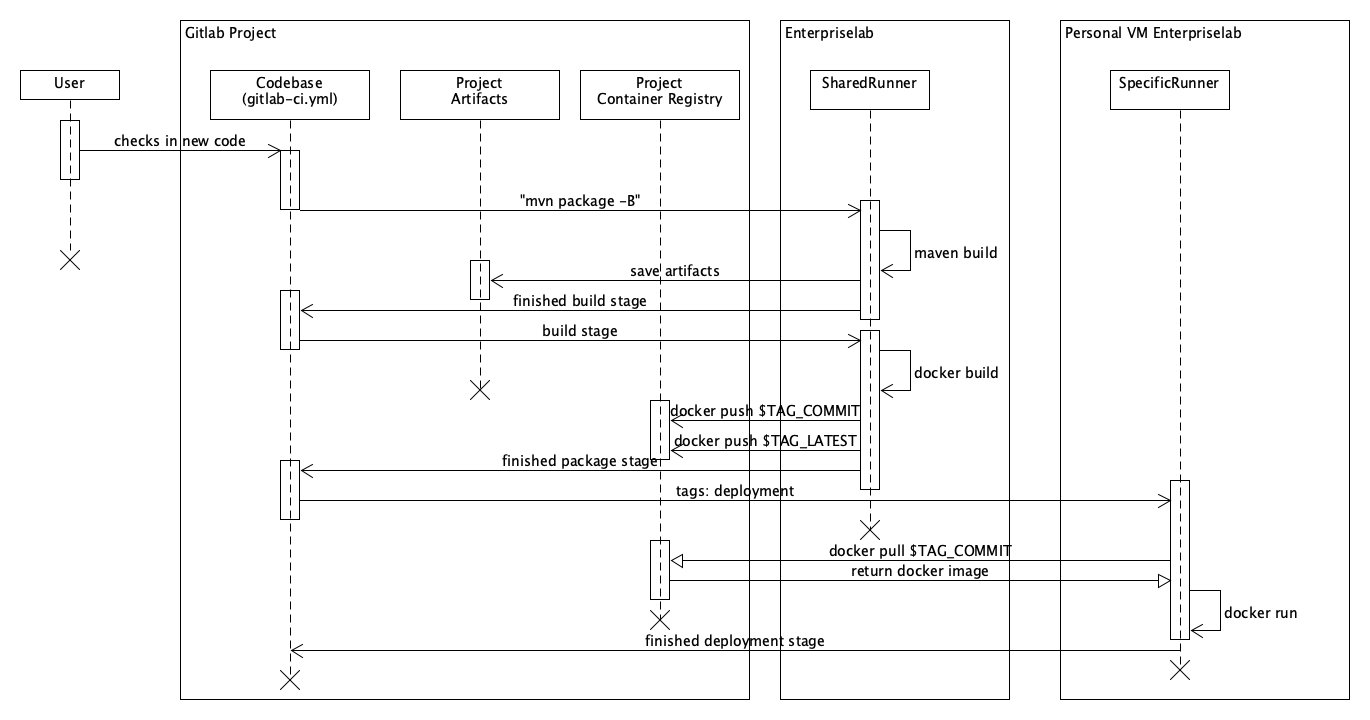
\includegraphics[width=1\textwidth]{images/sequenceCicd.png}
	\caption[Ablauf der CI/CD Pipeline]{Ablauf der CI/CD Pipeline,\\ Quelle: Autor}
	\label{img: cicdPipeline}
\end{figure}

\subsection{Testing}
Das Projektziel ist ein Prototyp. Aus diesem Grund wurde der Fokus auf die Funktion gesetzt. Daher wurden die Unit- und Integrationstests nur konzeptuell umgesetzt. Bei Bedarf können diese erweitert werden. 
\newpage